\documentclass{article}
\usepackage[utf8]{inputenc}
\usepackage{tkz-euclide}
\usepackage{graphicx}
\usepackage{hyperref}
\usepackage{amsmath}
\usepackage{amssymb}
\usepackage{tikz}
\usetkzobj{all}

\begin{document}

Convención del signo de los angulos

$\angle{QOP} > 0$
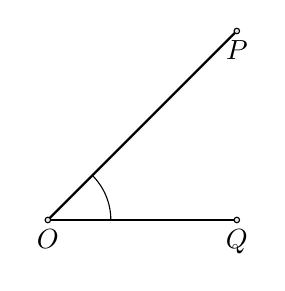
\begin{tikzpicture}[scale=.8]

% definitions
\tkzDefPoint(0,0){O}
\tkzDefPoint(3,3){P}
\tkzDefPoint(3,0){Q}
\tkzMarkAngle[label=QOP, size=1](Q,O,P)

\tkzDrawSegments[thick](O,P)
\tkzDrawSegments[thick](O,Q)
\tkzDrawPoints(O,P,Q)

% labels
\tkzLabelPoints(Q,O,P)
\end{tikzpicture}

$\angle{QOP} < 0$  o $\angle{QOP} > 12:00:00h $ (los angulos mayores de 180 grados se representan con valor negativo)
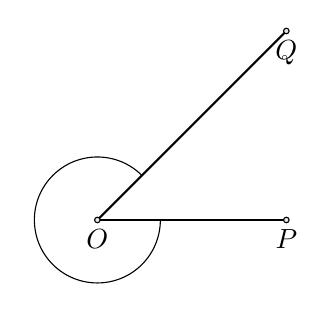
\begin{tikzpicture}[scale=.8]

% definitions
\tkzDefPoint(0,0){O}
\tkzDefPoint(3,3){Q}
\tkzDefPoint(3,0){P}
\tkzMarkAngle[label=QOP, size=1](Q,O,P)

\tkzDrawSegments[thick](O,P)
\tkzDrawSegments[thick](O,Q)
\tkzDrawPoints(O,P,Q)

% labels
\tkzLabelPoints(Q,O,P)
\end{tikzpicture}



\begin{itemize}
\item O: centro de la tierra y de la esfera celeste (esfera que contiene la esfera de la tierra, el plano ecuadorial terrestre se extiende al plano ecuadorial celeste y la comparte igual que la tierra en 2 hemisferios: norte y sur y el plano del meridiano 0 se puede extender para toda la esfera celeste). La correspondiente de la latitud en la tierra es la declinación para la esfera celeste (negativa si el objeto a observar está en hemisferio sur celeste) y para la longitud la declinación recta(positiva desde el meridiano 0 en el sentido de la rotación dela tierra en torno a su propio eje y negativa en el otro sentido)
\item P: punto del observador
\item T: posicion del objeto observado
\end{itemize}

Proyeccion longitudinal
P está en el hemisferio norte(latitud positiva) 
\vspace{5cm}


Declinacion negativa
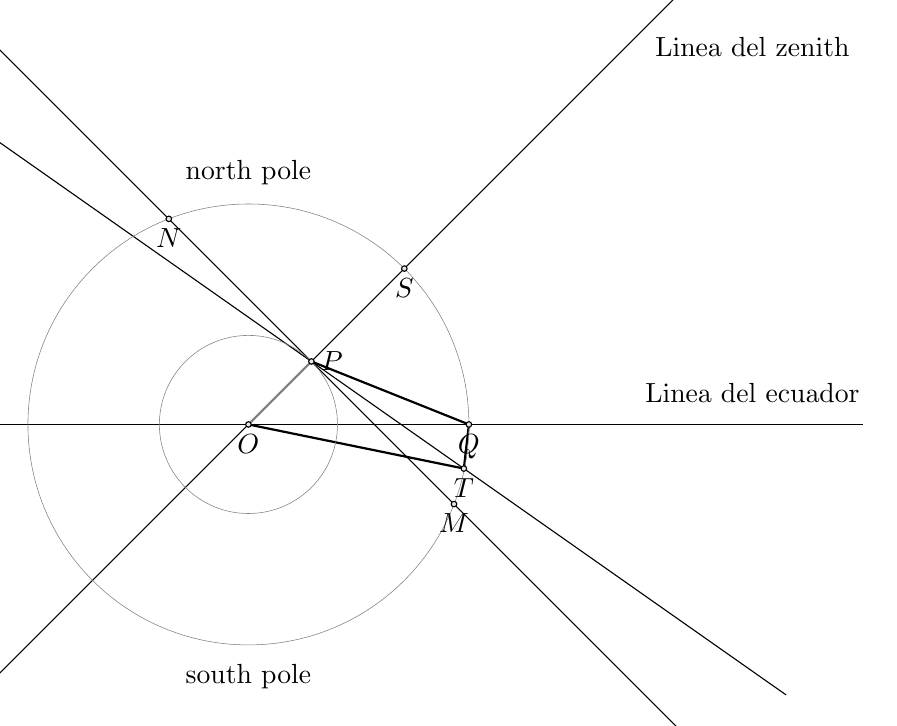
\begin{tikzpicture}[scale=.8]

% definitions
\tkzDefPoint(0,0){O}
\tkzDefPoint(1,1){P}
\tkzDefPoint(3.5,0){Q}
\tkzDefPoint(3.42,-0.7){T}

\tkzDefPointWith[orthogonal](P,O) \tkzGetPoint{P1} % find a point P1 orthogonal to PO
\tkzInterLC(P,P1)(O,Q) \tkzGetPoints{M}{N} % find intersections of a line passing through A and Q with the large circle 
\tkzInterLC(O,P)(O,Q) \tkzGetPoints{P4}{S} % find intersections of a line passing through A and Q with the large circle 
\draw [shorten >= -5cm, shorten <=-5cm] (P4)--(S);
\draw [shorten >= -5cm, shorten <=-5cm] (O)--(Q);
\node at (8,0.5){Linea del ecuador} ; 
\node at (8,6){Linea del zenith} ; 
\draw [shorten >= -5cm, shorten <=-5cm] (P)--(T) ;
\draw [shorten >= -5cm, shorten <=-5cm] (M)--(N) ;
%\tkzMarkAngle[label=lat, size=1](Q,O,P)

\tkzDrawSegments[thick](O,T)
\tkzDrawSegments[thick](T,Q)
\tkzDrawSegments[thick](P,Q)
%\tkzMarkAngle[](Q,O,T)
%\tkzMarkAngle[label=dec, size=1](Q,P,T)
%\tkzMarkAngle[label=zd, size=1](P4,P,T)
% drawing
\tkzDrawCircle(O,P)
\tkzDrawCircle(O,Q) 
\node at (0,4){north pole};
\node at (0,-4){south pole};
\tkzDrawSegments[thick,gray](O,P)
\tkzDrawPoints(O,P,Q,T,M,S,N)

% labels
\tkzLabelPoints(Q,T,O,M,S,N)
\tkzLabelPoints[right](P)
\end{tikzpicture}

\vspace{5cm}

Declinacion positiva
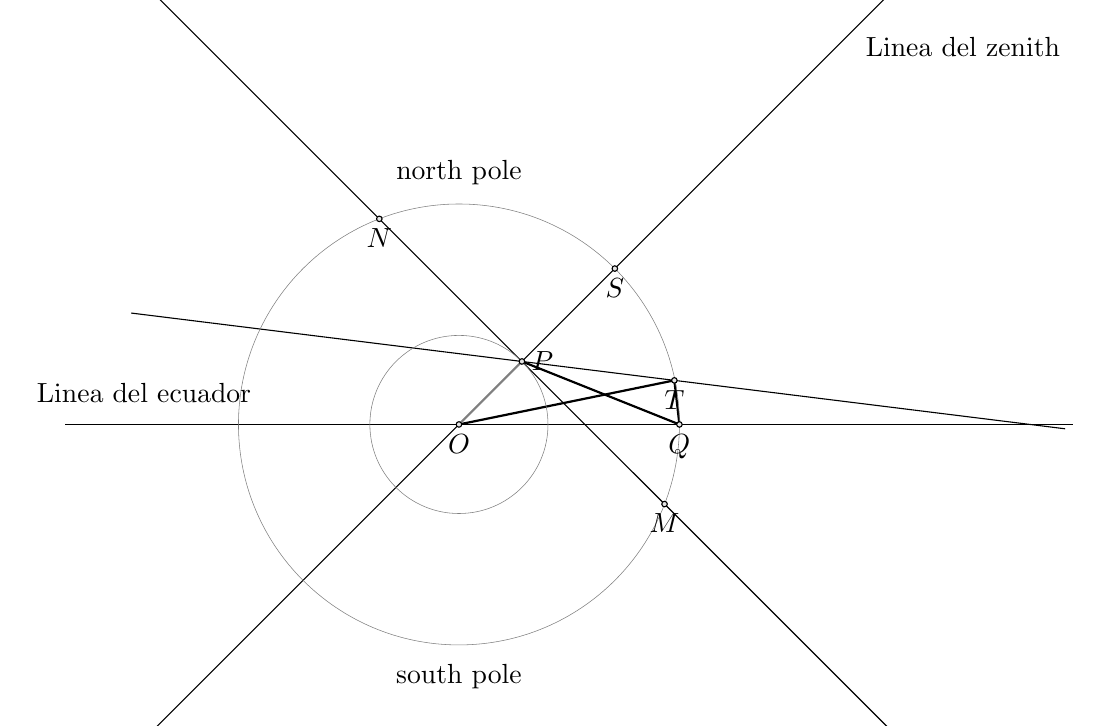
\begin{tikzpicture}[scale=.8]

% definitions
\tkzDefPoint(0,0){O}
\tkzDefPoint(1,1){P}
\tkzDefPoint(3.5,0){Q}
\tkzDefPoint(3.42,0.7){T}
\node at (-5,0.5){Linea del ecuador} ; 
\node at (8,6){Linea del zenith} ; 

\tkzDefPointWith[orthogonal](P,O) \tkzGetPoint{P1} % find a point P1 orthogonal to PO
\tkzInterLC(P,P1)(O,Q) \tkzGetPoints{M}{N} % find intersections of a line passing through A and Q with the large circle 
\tkzInterLC(O,P)(O,Q) \tkzGetPoints{P4}{S} % find intersections of a line passing through A and Q with the large circle 
\draw [shorten >= -5cm, shorten <=-5cm] (P4)--(S);
\draw [shorten >= -5cm, shorten <=-5cm] (O)--(Q) ;
\draw [shorten >= -5cm, shorten <=-5cm] (P)--(T) ;
\draw [shorten >= -5cm, shorten <=-5cm] (M)--(N) ;
%\tkzMarkAngle[label=lat, size=1](Q,O,P)

\tkzDrawSegments[thick](O,T)
\tkzDrawSegments[thick](T,Q)
\tkzDrawSegments[thick](P,Q)
%\tkzMarkAngle[](Q,O,T)
%\tkzMarkAngle[label=dec, size=1](Q,P,T)
%\tkzMarkAngle[label=zd, size=1](P4,P,T)
% drawing
\tkzDrawCircle(O,P)
\tkzDrawCircle(O,Q)
\node at (0,4){north pole};
\node at (0,-4){south pole};
\tkzDrawSegments[thick,gray](O,P)
\tkzDrawPoints(O,P,Q,T,M,S,N)

% labels
\tkzLabelPoints(Q,T,O,M,S,N)
\tkzLabelPoints[right](P)
\end{tikzpicture}


\vspace{5cm}
\begin{itemize}
\item OQ: linea del ecuador
\item OP: linea del zenit del observador(la linea que une el observador con el centro de la tierra) perpendicular en la linea del horizonte MN(solo se pueden ver objetos en el arco MSN: objetos con declinación entre -(90$^\circ$ - latitude) y 180$^\circ$ - (90$^\circ$ - latitude) )
\item PT: linea de vision del observador
\item $\angle{QPT}$ Para la proyeccion longitudinal es declinacion medida por el telescopio(negativa si la estrella está debajo del plano ecuadorial) - el angulo en el cielo entre la dirección del telescopio orientado hacia el objeto que observamos y la direccion del telescopio orientado hacía un objeto que está en el ecuador celeste. 
\item $\angle{QOT}$  declinacion  de la estrella (negativa si la estrella está debajo del plano ecuadorial) - medida desde un punto que esta en el ecuador de la tierra 
\item $\angle{QOP}$  latitud
\item $\angle{TPS}$  proyeccion en este plan del angulo zenith distance(formado por la linea del zenith y la direccion en cual apunta el telescopio) 
\item En práctica esta es zenith distance (el azimuth no cuenta) ZD medida en grados  (dd:mm:ss) con dd entre 00 y 90
y Airmass se aproxima como 1 / cos(ZD)


\end{itemize}
\begin{description}
\item $\angle{POQ} = \angle{POT} + \angle{TOQ}$
\item Q(el objeto de referrencia) está muy lejos asi que las distancias $OQ, PQ, PT, OT \gg OP$(el radio de la tierra) y  $\angle{TPQ}\approx \angle{TOQ} $ (la declinacion medida por el telescopio es aprox la declinacion del objeto observado medida desde un punto del ecuador terrestre si el objeto está bastante lejos)  	
\item Ademas si se apunta el telescopio cerca al zenith $\angle{SPT} \approx \angle{POT} \approx 0$ así que $\angle{POQ} \approx \angle{TPQ}$(latitud $\approx$ declinación)
\item Miramos las imagenes del flat del cielo (cuando el telescopio esta orientado aprox hacia el zenith) y determinamos la latitud 28:17:48
(grados)
\end{description}

Proyeccion transversal
P está al este del meridiano 0 terrestre(longitud positiva)

\vspace{5cm}

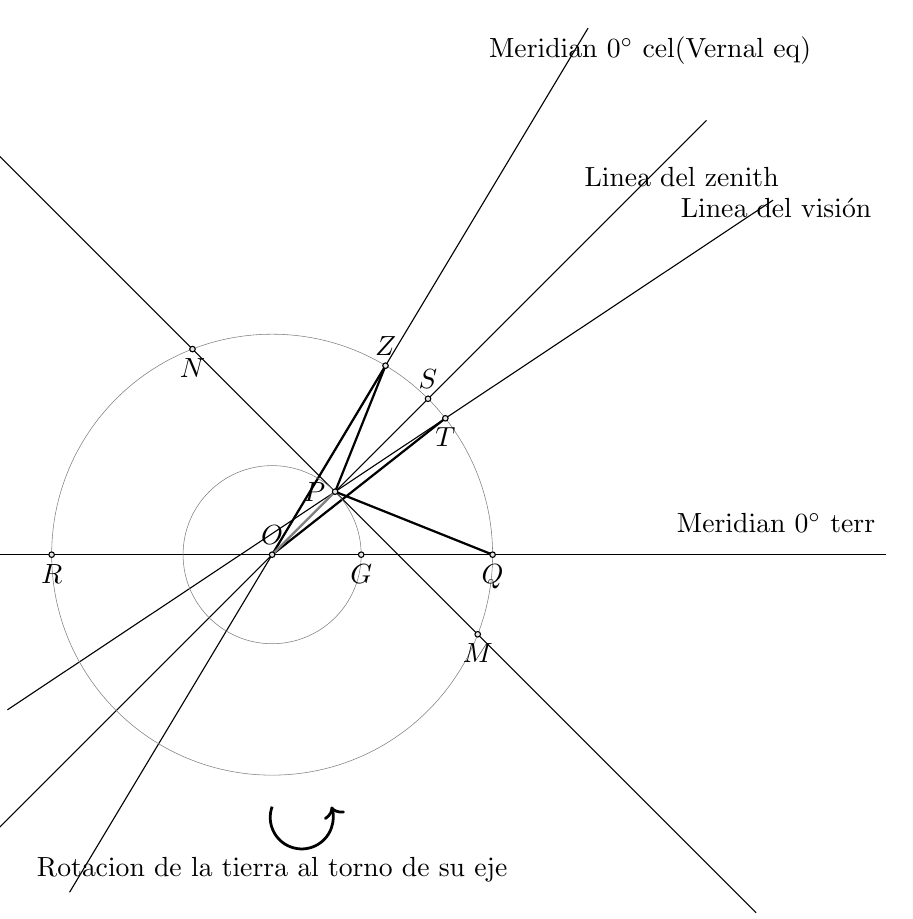
\begin{tikzpicture}[scale=.8]

% definitions
\tkzDefPoint(0,0){O}
\tkzDefPoint(1,1){P}
\tkzDefPoint(3.5,0){Q}
\tkzDefPoint(-3.5,0){R}
\tkzDefPoint(2.75,2.165){T}
\tkzDefPoint(1.8, 3){Z}
\node at (8,0.5){Meridian 0$^\circ$ terr} ; 
\node at (6,8){Meridian 0$^\circ$ cel(Vernal eq)} ; 
\node at (6.5,6){Linea del zenith} ; 
\node at (8,5.5){Linea del visión} ; 

\tkzDefPointWith[orthogonal](P,O) \tkzGetPoint{P1} % find a point P1 orthogonal to PO
\tkzInterLC(P,P1)(O,Q) \tkzGetPoints{M}{N} % find intersections of a line passing through A and Q with the large circle 
\tkzInterLC(O,P)(O,Q) \tkzGetPoints{P4}{S} % find intersections of a line passing through A and Q with the large circle 
\tkzInterLC(Q,R)(O,P) \tkzGetPoints{G}{P5} % find intersections of a line passing through A and Q with the large circle 
\draw [shorten >= -5cm, shorten <=-5cm] (P4)--(S);
\draw [shorten >= -5cm, shorten <=-5cm] (O)--(Q) ;
\draw [shorten >= -5cm, shorten <=-5cm] (O)--(Z) ;
\draw [shorten >= -5cm, shorten <=-5cm] (P)--(T) ;
\draw [shorten >= -5cm, shorten <=-5cm] (M)--(N) ;
%\tkzMarkAngle[label=lat, size=1](Q,O,P)

%\tkzDrawSegments[thick](O,T)
%\tkzDrawSegments[thick](T,Q)
\tkzDrawSegments[thick](P,Q)
\tkzDrawSegments[thick](P,Z)
\tkzDrawSegments[thick](O,Z)
\tkzDrawSegments[thick](O,T)
%\tkzMarkAngle[](Q,O,T)
%\tkzMarkAngle[label=dec, size=1](Q,P,T)
%\tkzMarkAngle[label=zd, size=1](P4,P,T)
% drawing
\tkzDrawCircle(O,P)
\tkzDrawCircle(O,Q)
\draw [->,line width=1pt] (0,-4) arc[x radius=0.5cm, y radius =.5cm, start angle=-200, end angle=20];
\node at (0,-5){Rotacion de la tierra al torno de su eje} ; 
\tkzDrawSegments[thick,gray](O,P)
\tkzDrawPoints(O,P,Q,T,M,S,N,Z,R,G)

% labels
\tkzLabelPoints(Q,T,M,N,R,G)
\tkzLabelPoints[left](P)
\tkzLabelPoints[above](O,Z,S)
\end{tikzpicture}

\vspace{5cm}
\begin{itemize}
\item Z vernal equinox
\item G punto en la tierra en el meridiano 0
\item $\angle{ZOQ}$ UniversalTime
\item $\angle{ZPT} \approx \angle{ZOT}$ RightAscension
\item $\angle{ZPS} \approx \angle{ZOS}$ SiderealTime
\item $\angle{SPT} \approx \angle{SOT}$ object hour
\item (ST = RA + h), cuando el objeto a observar está justo arriba(h=0) ST = RA
\item $\angle{QOP}$ longitud
\end{itemize}


\begin{description}
\item Cuando Sidereal Time es aprox 0 UT representa la longitud
\item longitud 22:21:45(hours) = -24:34:45(degrees)    

\end{description}

\subsection*{Instrumento}
\url{http://www.ing.iac.es/astronomy/instruments/wfc/index.html}

\subsection*{Noise}
En los headers de las imagenes(y en la especificacion de la pagina web para exposisiones largas(48 sec) - exposiciones cortas(29 sec)):
\begin{description}
\item GAIN    =                   2.  /  gain, electrons per adu (1.26 - 2.5)
\item RDNOISE =                  5.4  /  read noise, electrons (4.6 - 9)
\end{description}

En la pagina web:
\begin{description}
\item Noise(ADU) (3.7 - 3.6)
\item Bias (2030 - 1830)
\end{description}

\subsection*{Field of view and detector size}
En la pagina web:
\begin{description}
\item Field of View 34x34arcmin
\item Pixel scale 0.333 arcsec / pixel
\item pixel size = 13.5 microns
\end{description}


\begin{description}
\item Numero de pixeles del detector = FOV / pixel scale = 6126 x 6126, diferente al numero de pixeles por filas y columnas del header de las imagenes fits 
\item tamaño del detector = num pixeles * pixel size = 82.7 mm
\end{description}


\subsection*{Reducción de las imagenes}
\begin{itemize}
\item
Separar las imagenes en carpetas por tipo: object y flat y cada una por el fitro(B, R, V) (función initDirs() in red.py)
\item
Correción bias(sustraer bias de la imagen): con la función colbias de iraf(función trimAndOverscan() in red.py): se calcula una columna como media de las columnas definidas en la sección bias y se sustrae de todas las columnas de la sección trim. Se hace para todas las imagenes: flat y object
\item 
Crear los ficheros flat que se usan para la correción de flat:
con imcombine se hace una media de todas las imaganes flat para cada filtro y despues se normalizan dividiendo por la media(mean) de cada uno (usando la función iraf imarith) (función createFlatFiles() en red.py)
\item
Correción de flat:
Todas las imagenes tipo object se dividen con el flat medio normalizado para cada filtro (función flatCorrection() en red.py)
\item para la fotometría elegimos solo la parte central del cúmulo (las imagenes que tienen los últimos 3 dígitos antes de la extensión .fits  formando un número $ \in  [96,105] $)

\item corregir pixeles malos (independientes del filtro):
de forma aproximadamente automática: elegimos 2 flat con tiempo de exposition largo (EXPTIME keyword in header)
M37New/flat/V/Nov30032.fits (60) y M37New/flat/R/Nov30031.fits (35) y hacemos la media con imcombine
y 2 con el valor  EXPTIME pequeño: M37New/flat/V/Nov30016.fits (2)  M37New/flat/V/Nov30015.fits (2)
Luego dividimos los 2 resultados y creamos una mascara con ccdmask. Despues ejecutamos fixpix para lodas las imagenes tipo object y el fichero mask obtenido antes:

\begin{verbatim}

ecl> imcombine M37New/flat/R/Nov30031.fits,M37New/flat/V/Nov30032.fits M37New/flat/FlatBigExptime
ecl> imcombine M37New/flat/V/Nov30016.fits,M37New/flat/V/Nov30015.fits M37New/flat/FlatSmallExptime
ecl> imarith  M37New/flat/FlatBigExptime /  M37New/flat/FlatSmallExptime  M37New/flat/FlatBigSmallDivided
ecl> noao
ecl> imred
ecl> ccdred
ecl> ccdmask  M37New/flat/FlatBigSmallDivided  M37New/flat/MaskFile 
ecl> cd M37New/object/V
ecl> fixpix @list /scratch1/tobs/M37New/flat/MaskFile
ecl> cd ../R
ecl> fixpix @list /scratch1/tobs/M37New/flat/MaskFile
ecl> cd ../B
ecl> fixpix @list /scratch1/tobs/M37New/flat/MaskFile


\end{verbatim}

\item Si queremos definir una mascara:

Si miramos en la imagen  Nov30098.fits y queremos definir en la columna 577($ x \in [577,578) $) como pixeles malos la parte de abajo ($ y \in [0, 259) $)
\begin{verbatim}
bpopescu@colibri:/scratch1/tobs$ cat col577Mask 
box 577 0 578 259
\end{verbatim}

\begin{verbatim}
ecl> mskregions.regions="col577Mask"
ecl> mskregions.dims="1024,1024"
ecl> mskregions.masks="M37New/flat/Col577Mask"
ecl> mskregions.refimages="M37New/object/V/Nov30098.fits"
ecl> mskregions
The list of region specifications (col577Mask): 
The list of output mask images (M37New/flat/Col577Mask): 
The list of input reference images (M37New/object/V/Nov30098.fits): 
Creating mask M37New/flat/Col577Mask.pl using reference image M37New/object/V/Nov30098.fits
    Using regions file col577Mask
ecl> 
\end{verbatim}
(Si no queremos que nos pregunte siempre por los parametros hay que modificar el parametro mode del task de 'ql' a 'h')

Se crea un fichero /scratch1/tobs/M37New/flat/Col577Mask.pl, no hace falta especificar la extensión .pl en el paso siguiente cuando se pasa como parametro al task fixpix:

Después hay que modificar todas las imagenes tipo object con fixpix como antes


\begin{verbatim}
ecl> cd M37New/object/V
ecl> fixpix @list /scratch1/tobs/M37New/flat/Col577Mask
ecl> cd ../R
ecl> fixpix @list /scratch1/tobs/M37New/flat/Col577Mask
ecl> cd ../B
ecl> fixpix @list /scratch1/tobs/M37New/flat/Col577Mask
\end{verbatim}

Miramos la diferencia entre las imagenes antes de aplicar esta mascara y despues:
			
\begin{verbatim}

        cl> display.xsize=0.5
        cl> display M37New/object/V/Nov30098.fits fill+ xcen=0.25
        cl> display Nov30098.fits erase- fill+ xcen=0.75


\end{verbatim}

\begin{figure}[!ht]
 \centering
 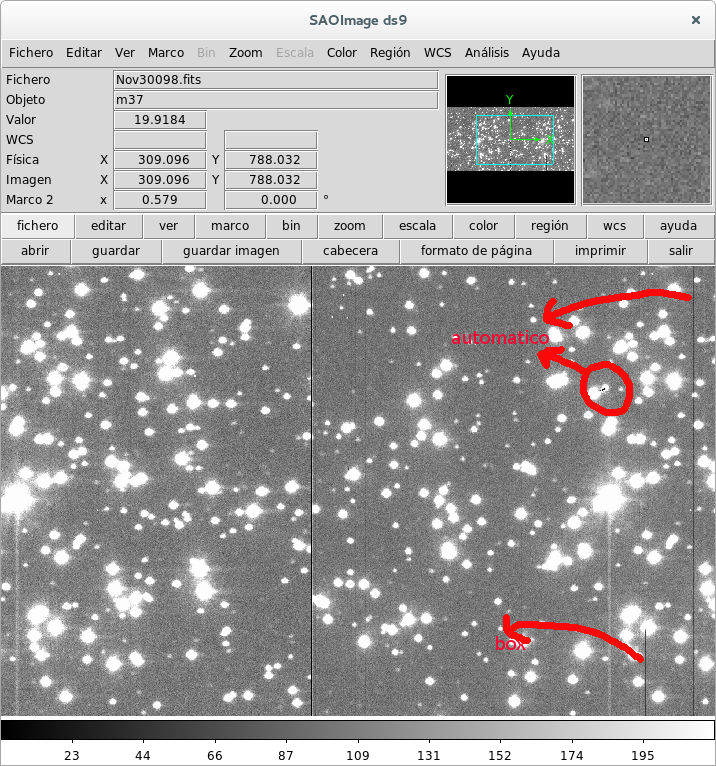
\includegraphics[scale=0.5]{fixpix.png}
 \caption{\emph{Perfil radial de las estrellas de referencia para la alineación}}
\end{figure}


\item
FOTOMETRIA:
Alinear las imagenes:
Se elige una imagen con buena respuesta elegí Nov30098.fits en filtro V y 3 estrellas bien separadas en la imagen que no tengan mucho ruido y que no estén saturadas

\begin{figure}[!ht]
 \centering
 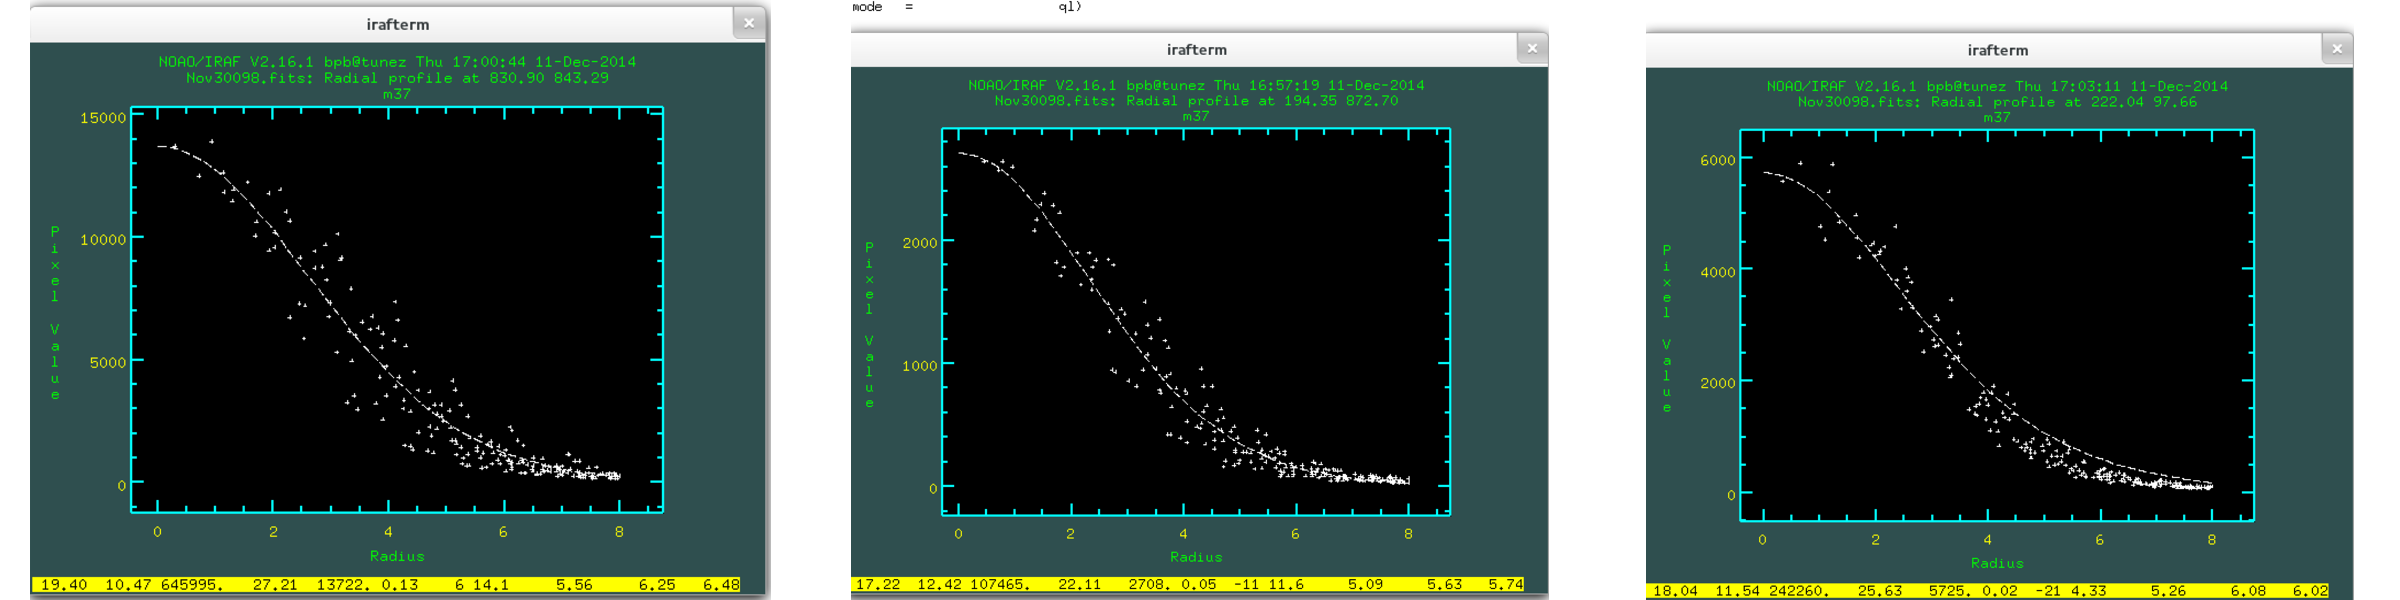
\includegraphics[scale=0.2]{align_rp.png}
 \caption{\emph{Perfil radial de las estrellas de referencia para la alineación}}
\end{figure}

\begin{verbatim}
para ver el perfil radial:
en xgterm abrir el visualizador ds9 (funciona con ximtool, pero no he probado)
en iraf
 ecl>display image.fits
 ecl>imexam image.fits
hacer click en el punto donde quieres ver el perfil radial y pulsar "r" después
\end{verbatim}


\item  escribir las coordenadas en un fichero
\begin{verbatim}
[bpopescu@colibri tobs]$ cat coords-98.txt
194 872
831 843
222 98
\end{verbatim}

\item Usamos imcentroid para obtener las coordenadas exactas usando como input la misma imagen de referencia

\begin{verbatim}

        ecl> imcentroid.input = "M37New/object/V/Nov30098.fits" 
	    	ecl> imcentroid.reference = "M37New/object/V/Nov30098.fits" 
       	ecl> imcentroid.coords = "coords-98.txt"
				ecl> imcentroid

salen las coordenadas:

#Coords        Image     X-center   Err      Y-center   Err     Num
/scratch/M37New/object/V/Nov30098.fits     194.519 (0.028)     872.795 (0.024)     1
/scratch/M37New/object/V/Nov30098.fits     830.926 (0.015)     843.310 (0.010)     2
/scratch/M37New/object/V/Nov30098.fits     222.031 (0.018)      97.730 (0.019)     3

#Refcoords Reference     X-center   Err      Y-center   Err     Num
/scratch/M37New/object/V/Nov30098.fits     194.519 (0.028)     872.795 (0.024)     1
/scratch/M37New/object/V/Nov30098.fits     830.926 (0.015)     843.310 (0.010)     2
/scratch/M37New/object/V/Nov30098.fits     222.031 (0.018)      97.730 (0.019)     3

#Shifts        Image    X-shift   Err      Y-shift   Err      N      Internal
/scratch/M37New/object/V/Nov30098.fits      0.000 (0.017)      0.000 (0.015)    3   (0.000,0.000)

miramos los nuevos valores de x-center y y-center y los ponemos en otro fichero:

[bpopescu@colibri tobs]$ cat coords-98-aligned.txt 
194.519 872.795
830.926 843.310
222.031 97.730


\end{verbatim}

\item Alinear lodas las imagenes: usando imalign
Creamos una lista(fichero listCenter) con las imagenes  que hay que alinear(las tipo "object" del centro del cúmulo (con el numero del nombre  de 96 a 105)) y otra a cual añadimos 'a' antes de la extensión (fichero listCenterAligned) con alignImages.py (ejecutando align desde pyraf, sale un error, porque?)

\begin{verbatim}
 	ecl>      imalign.input="@listCenter"   
  ecl>  		imalign.reference = "M37New/object/V/Nov30098.fits" 
  ecl>     	imalign.coords = "coords-98-aligned.txt" 
  ecl>    	imalign.output = "@listCenterAligned" 
  ecl>    	imalign.interp_type = "nearest" 
	ecl>			imalign
\end{verbatim}

\item 


\end{itemize}



\subsection*{Observaciones}
\begin{itemize}
\item eliminar pixeles malos: ccdmask
De fornma adicional quiero aplicar otro mask y quiero definir columnas 660 y 678 como columnas malas(para corregir por ejemplo img 65) y uso un fichero mask de forma:
\begin{verbatim}
cols (660,660) || cols (678,678) ? 1 : 0
\end{verbatim}
pero sale un error: "segmentation violation". Pero funciona con un fichero mask definido:
\begin{verbatim}
circle (220., 220., 50.) && circle (240., 220., 50.) ? 1 : 0
\end{verbatim}





\end{itemize}

\end{document}
